We will now examine the details of monoclonal antibody production.
It is done in multiple steps, as summarized on figure \ref{fig:Monoclonal_Antibody_Production}.

\begin{figure}[H]
    \begin{center}
        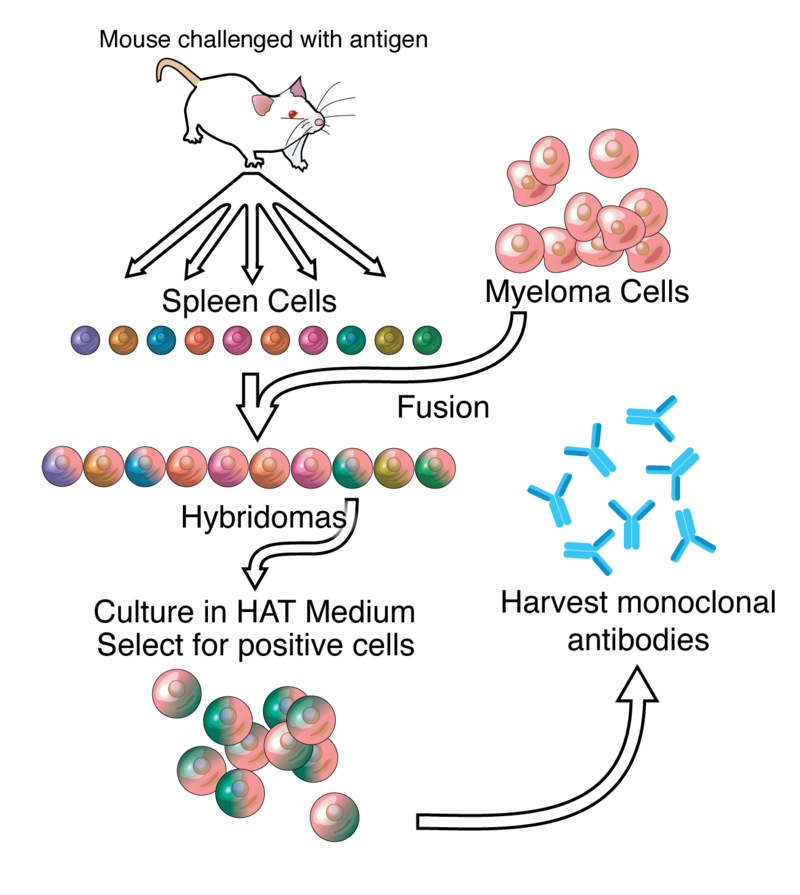
\includegraphics[width=0.4\textwidth]{../Images/mab_hybridomas.png}
        \caption{Monoclonal antibody production}
        \label{fig:Monoclonal_Antibody_Production}
    \end{center}
\end{figure}


\subsubsection{Step 1 : Immunization}

In order to begin the production of monoclonal antibodies, it is first
needed to immunize an animal with the antigen of interest. Typically, 
mice are used for this process \cite{leenaars_critical_2005}. 
An \emph{immunogen}, \textit{i.e} an antigen due to induce an immune response
in the animal, is then injected into the animal, along with an adjuvant
aiming at enhancing the immune response.


\subsubsection{Step 2 : Fusion and selection}

\subsubsection{Step 3 : Screening}

\subsubsection{Step 4 : Characterization}

\subsubsection{Step 5 : Production}